% --------------------------------------------------------------------------------
% --------------------------------------------------------------------------------
% Projeto de Pesquisa realizado para Conclusão da Graduação em Psicologia
% Acadêmico: Bruno Braga Montezano
% Baseia-se no documento modelo de Projeto de Pesquisa do abnTeX2
% --------------------------------------------------------------------------------
% --------------------------------------------------------------------------------

% ------------------------
% Preâmbulo do Documento
% ------------------------

\documentclass[chapter=TITLE,
               oneside,
               12pt,
               a4paper,
               english,
               brazil]{abntex2}    % Opções comuns: [openright,twoside,a4paper,brazil]

\titulo{Efeitos do prejuízo no sono na
        funcionalidade e cognição de
        sujeitos com transtornos de humor}

\autor{Bruno Braga Montezano}

\instituicao{Universidade Católica de Pelotas}

\local{Pelotas}

\orientador[Prof\textsuperscript{a}. Dra.]{Karen Jansen}

\preambulo{Projeto de Pesquisa apresentado à
           Universidade Católica de Pelotas,
           como parte das exigências para a aprovação na
           disciplina Trabalho de Conclusão em Psicologia I}

% ---------------------------------
% Pacotes Utilizados no Trabalho
% ---------------------------------

\usepackage[backend=biber,
            style=abnt,
            uniquename=init,
            giveninits,
            repeatfields]{biblatex} % Citações padrão ABNT

\addbibresource{ref.bib}            % Adicionando arquivo de bibliografia

\usepackage[utf8]{inputenc}         % Suporte para codificação UTF-8
\usepackage[T1]{fontenc}            % Suporte para codificação de fonte T1

\usepackage{indentfirst}            % Indenta o primeiro parágrafo de cada seção
\usepackage{nameref}                % Permite referenciar nome de uma seção

\usepackage{graphicx}               % Pacote para inserir imagens e tabelas
\usepackage{pdfpages}               % Pacote para inserir páginas em PDF
\usepackage{lscape}                 % Pacote para modo paisagem

\usepackage{newtxtext,newtxmath}    % Pacotes para utilizar Times
\usepackage{microtype}              % Melhorar aparência sem obstrução visual
\usepackage[font=sf]{caption}       % Legenda com fonte sem serifa

\usepackage{booktabs}               % Pacote para criar tabelas no estilo booktabs
\usepackage{longtable}              % Pacote para criar tabelas de múltiplas páginas
\usepackage{tabu}                   % Pacote para flexibilizar tabelas e tabelas longas
\usepackage{array}                  % Pacote para ampliar opções de formatos de coluna
\usepackage{float}                  % Pacote para flutuar elementos
    \floatstyle{plaintop}           % Força legenda das tabelas no topo
    \restylefloat{table}            % Deixa as tabelas flutuantes


% -------------------------------------
% Modificações na Classe de Documento
% -------------------------------------

% Modificando fonte do documento para fonte sem serifa

\renewcommand{\familydefault}{\sfdefault} % Fonte padrão do documento para sem serifa
\urlstyle{same}                           % URLs com mesma fonte do corpo do texto

% Modificando indentação e espaçamento entre títulos

\setlength{\parindent}{1.3cm}
\setlength{\parskip}{0.2cm}
\setlength{\afterchapskip}{10pt}
\setlength{\beforechapskip}{20pt}
\setlength{\midchapskip}{20pt}
\setlength{\beforesecskip}{20pt}
\setlength{\aftersecskip}{10pt}

% Modificando o tamanho da fonte dos capítulos e seções

\renewcommand{\ABNTEXchapterfont}{\normalfont\fontseries{b}\selectfont}
\renewcommand{\ABNTEXchapterfontsize}{\normalsize}
\renewcommand{\ABNTEXpartfont}{\fontseries{b}\selectfont\selectfont}
\renewcommand{\ABNTEXpartfontsize}{\normalsize}
%\renewcommand{\ABNTEXsectionfont}{\normalfont\selectfont}
\renewcommand{\ABNTEXsectionfont}{\normalfont\fontseries{b}\selectfont}
\renewcommand{\ABNTEXsectionfontsize}{\normalsize}
%\renewcommand{\ABNTEXsubsectionfont}{\normalfont\fontseries{b}\selectfont}
\renewcommand{\ABNTEXsubsectionfont}{\normalfont\fontseries{b}\itshape\selectfont}
\renewcommand{\ABNTEXsubsectionfontsize}{\normalsize}
\renewcommand{\ABNTEXsubsubsectionfont}{\normalfont\selectfont}
\renewcommand{\ABNTEXsubsubsectionfontsize}{\normalsize}
\renewcommand{\ABNTEXsubsubsubsectionfont}{\normalfont\itshape\selectfont}
\renewcommand{\ABNTEXsubsubsubsectionfontsize}{\normalsize}

% Modificando a capa aos padrões da UCPel

\renewcommand{\imprimircapa}{%
    \begin{capa}%
        \center
        \ABNTEXchapterfont\Large\MakeUppercase\imprimirinstituicao

        \vspace*{1cm}

        {\ABNTEXchapterfont\Large\MakeUppercase\imprimirautor}

        \vfill
        \begin{center}
            \ABNTEXchapterfont\bfseries\LARGE\MakeUppercase\imprimirtitulo
        \end{center}
        \vfill

        \large\imprimirlocal

        \large{2020}

        \vspace*{1cm}
    \end{capa}
}

% Modificando a folha de rosto aos padrões da UCPel

\makeatletter
\renewcommand{\folhaderostocontent}{
\begin{center}
    {\ABNTEXchapterfont\Large\MakeUppercase\imprimirautor}


    \vspace*{\fill}\vspace*{\fill}
    \begin{center}
    \ABNTEXchapterfont\bfseries\Large\MakeUppercase\imprimirtitulo
    \end{center}
    \vspace*{\fill}

    \abntex@ifnotempty{\imprimirpreambulo}{%
        \hspace{.45\textwidth}
        \begin{minipage}{.5\textwidth}
            \SingleSpacing
            \large\imprimirpreambulo
        \end{minipage}%
        \vspace*{\fill}
    }%

    \hfill{\large{Orientadora: \imprimirorientadorRotulo~\imprimirorientador\par}}
    \abntex@ifnotempty{\imprimircoorientador}{%
        {\large\imprimircoorientadorRotulo~\imprimircoorientador}%
    }%
    \vspace*{\fill}

    \bfseries\large\imprimirlocal
    \par
    \bfseries\large{2020}
    \vspace*{1cm}

\end{center}
}

% ---------------------
% Início do Documento
% ---------------------

\begin{document}

\imprimircapa

\imprimirfolhaderosto

\pretextualchapter{Identificação}\label{sec:identificacao}

    \begin{itemize}

        \item \textbf{Título:} \imprimirtitulo

        \item \textbf{Discente:} \imprimirautor

        \item \textbf{Orientador:} \imprimirorientadorRotulo~\imprimirorientador

        \item \textbf{Instituição:} \imprimirinstituicao
            
        \item \textbf{Centro:} Centro de Ciências da Saúde

        \item \textbf{Curso:} Psicologia

        \item \textbf{Data:} Outubro, 2020

    \end{itemize}

\newpage
\begin{KeepFromToc}
\tableofcontents
\end{KeepFromToc}
\newpage

\begin{resumo}

    Há evidências que o sono está relacionado com a conversão diagnóstica
    e pior funcionamento e desempenho cognitivo em amostras tardias com
    transtornos de humor.
    Porém não se sabe o efeito do sono nessas medidas em amostras de sujeitos
    recém diagnosticados com TB.
    Este estudo trata-se de um estudo longitudinal com amostra de adultos entre
    18 e 60 anos diagnosticados com transtorno depressivo maior (n = 585) na
    cidade de Pelotas - RS. Os sujeitos foram reavaliados após dois anos para
    verificação do quadro diagnóstico e medidas de funcionamento e cognição.
    Para a observação do funcionamento, foi utilizada a escala
    \textit{Functioning Assessment Short Test} (FAST). Na aferição da cognição,
    verificou-se uma medida subjetiva, através da
    \textit{Cognitive Complaints in Bipolar Disorder Rating Assessment} (COBRA),
    e uma medida objetiva com o subteste Sequência de Números e Letras da
    \textit{Wechsler Adult Intelligence Scale}.
    Espera-se encontrar como resultado que a insônia/hipersonia se apresentará
    como um preditor para conversão, além de observar que mesmo em amostras
    recém diagnosticadas com TB, o sono já estará relacionado com prejuízo
    cognitivo e funcional.
    Sendo assim, o objetivo do estudo é avaliar o efeito da
    insônia/hipersonia na funcionalidade e cognição de sujeitos com
    transtornos de humor.

    \vspace{\onelineskip}

    \textbf{Palavras-chave:} transtorno bipolar; insônia; hipersonia;
    funcionamento cognitivo; adultos jovens.

\end{resumo}

\textual

\begingroup
\renewcommand{\cleardoublepage}{}
\renewcommand{\clearpage}{}

\chapter{Introdução}\label{sec:introducao}
    
    O transtorno bipolar (TB) é um transtorno psiquiátrico severo e crônico,
    caracterizado por episódios depressivos, maníacos e mistos.
    O TB pode causar diversas consequências funcionais, no campo da cognição,
    profissional, interpessoal, entre outros.
    A recuperação funcional se mostra muito menor do que a recuperação dos
    sintomas, causando impactos mais duradouros ao indivíduo.
    \parencite{american_psychiatric_association_diagnostic_2013}.
    
    Na literatura, percebe-se uma grande associação entre as alterações do sono
    e os transtornos de humor.
    Os problemas no sono podem inclusive predizer o início do TB e do transtorno
    depressivo maior (TDM), tal como a recorrência de episódios de humor
    \parencite{melo_sleep_2016,
    kaplan_sleep_2020,
    andrade-gonzalez_initial_2020}.
    Essas alterações são percebidas também em pacientes em período de eutimia
    ou remissão
    \parencite{de_la_fuente-tomas_sleep_2018}.

    Alguns estudos relacionam as alterações do sono ao prejuízo no funcionamento
    e desempenho cognitivo de sujeitos com transtorno de humor
    \parencite{reyes_functional_2017,
    kapczinski_cognition_2016}.
    Os estudos que vêm examinando a respeito do efeito das perturbações no
    sono no funcionamento, verificam um prejuízo funcional maior em sujeitos
    com a presença desses problemas no sono. Além disso, um pior sono pode
    predizer um maior prejuízo no funcionamento
    \parencite{walz_daytime_2013,
    lai_familiality_2014,
    slyepchenko_association_2019}.

    Tal como no funcionamento, trabalhos que analisam a relação entre
    sono e desempenho cognitivo tendem a observar um pior sono associado
    a um pior desempenho cognitivo no sujeito afetado
    \parencite{russo_relationship_2015,
    kaplan_sleep_2020}.
    Ademais, alterações relacionadas ao sono, como variabilidade do sono,
    podem predizer uma pior memória de trabalho e desempenho no aprendizado
    verbal
    \parencite{kanady_association_2017}.

    Grande parte dos estudos avaliam amostras tardias, com pacientes diagnosticados
    há algum tempo com os transtornos observados.
    Portanto, os efeitos do prejuízo no sono no funcionamento e cognição podem
    ser equivocadamente aferidos por decorrência do impacto da neuroprogressão
    nos transtornos mentais
    \parencite{tohen_two-year_2000}.
    Para mais, a maioria dos trabalhos na literatura que avaliaram a cognição
    em amostras de sujeitos com transtornos de humor consideraram medidas
    objetivas. Este estudo busca avaliar o construto tanto de forma objetiva
    quanto subjetiva, considerando as possíveis inconsistências entre os critérios.
    
    Dado isto, vê-se importante mais estudos que possam verificar se existem efeitos
    do sono no prejuízo funcional e cognitivo em amostras recém diagnosticadas
    de TB e TDM, ou estas implicações se mostram somente em amostras mais
    tardias e prejudicadas.
    Considerando estes aspectos, o presente trabalho visa avaliar o efeito da
    insônia/hipersonia na funcionalidade e cognição de sujeitos com transtorno
    bipolar, transtorno depressivo maior recorrente e transtorno depressivo maior
    em remissão.

\vspace{\onelineskip}
\chapter{Objetivos}\label{sec:objetivos}

    \section{Objetivo Geral}\label{sec:geral}
    
        \begin{alineas}
    
            \item Avaliar o efeito da insônia/hipersonia na funcionalidade e
            cognição de sujeitos com transtornos de humor;
    
        \end{alineas}
    
    \section{Objetivos Específicos}\label{sec:especifico}
    
        \begin{alineas}[resume]
    
            \item Avaliar a qualidade do sono de sujeitos que converteram para TB
            quando comparados aos sujeitos com episódio depressivo recorrente ou
            persistente e sujeitos que apresentaram remissão;
    
            \item Comparar o tempo de sono total entre sujeitos que converteram para
            TB, sujeitos com episódio depressivo recorrente ou persistente e sujeitos
            que apresentaram remissão;
    
            \item Comparar o escore de disfunções cognitivas entre sujeitos que
            converteram para TB, sujeitos com episódio depressivo recorrente ou
            persistente e sujeitos que apresentaram remissão;
    
            \item Comparar a percepção subjetiva de funcionamento cognitivo entre
            sujeitos que converteram para TB, sujeitos com episódio depressivo
            recorrente ou persistente e sujeitos que apresentaram remissão;
    
            \item Avaliar o efeito da insônia/hipersonia na conversão do
            diagnóstico de TDM para TB.
    
        \end{alineas}

\vspace{\onelineskip}
\chapter{Hipóteses}\label{sec:hipoteses}

    \begin{alineas}

        \item Os sujeitos bipolares apresentarão uma pior qualidade do sono
        quando comparados aos sujeitos que apresentam episódio depressivo
        recorrente ou persistente e sujeitos em remissão;

        \item Os sujeitos bipolares apresentarão um menor tempo de sono total
        quando comparados aos sujeitos que apresentam episódio depressivo
        recorrente ou persistente e sujeitos em remissão;

        \item Os sujeitos com episódio depressivo recorrente ou persistente
        apresentarão um maior escore de disfunções cognitivas quando comparados
        aos sujeitos bipolares;

        \item Os sujeitos com episódio depressivo recorrente ou persistente
        apresentarão uma maior incapacidade percebida no domínio de
        funcionamento cognitivo quando comparados aos sujeitos bipolares;

        \item A presença de insônia/hipersonia se apresentará como preditor
        para conversão de TDM para TB.

    \end{alineas}

\vspace{\onelineskip}
\chapter{Revisão de Literatura}\label{sec:revisao}

    \section{Estratégias de busca}\label{sec:estrategias}

        Esta revisão de literatura foi elaborada na base de dados do \textit{Pubmed}
        e da Biblioteca Virtual em Saúde (BVS), ambas no período entre setembro e
        outubro de 2020.
        Os descritores utilizados foram: \textit{``bipolar disorder''};
        \textit{``cognitive functioning''}; \textit{``cognitive impairment''};
        \textit{``cognitive performance''}; \textit{``depression''};
        \textit{``hypersomnia''}; \textit{``insomnia''}; \textit{``prodrome''};
        \textit{``recurrence''}; \textit{``relapse''}; \textit{``sleep dysfunction''};
        \textit{``sleep quality''}.
        Os resultados das combinações dos descritores está descrita nas tabelas
        \ref{tab:pubmed} e \ref{tab:bvs}.
    
        \begin{table}[H]
        \resizebox{\textwidth}{!}{%
            \caption{Descrição das estratégias de buscas na base de dados
            do \textit{Pubmed}}
            \label{tab:pubmed}
            \begin{tabular}{@{}p{0.4\textwidth}cccc@{}}
                \toprule
                    \textbf{Combinação dos descritores} &
                    \textbf{Artigos encontrados} &
                    \textbf{Títulos lidos} &
                    \textbf{Resumos lidos} &
                    \textbf{Artigos incluídos} \\ \midrule
                    \textit{sleep quality} \textbf{AND}
                    \textit{cognitive impairment} \textbf{AND}
                    \textit{bipolar disorder} &
                    18 & 7 & 5 & 4 \\ \midrule
                    \textit{insomnia} \textbf{AND} \textit{cognitive impairment}
                    \textbf{AND} \textit{bipolar disorder} &
                    16 & 5 & 4 & 4 \\ \midrule
                    \textit{sleep quality} \textbf{AND}
                    \textit{cognitive functioning} \textbf{AND}
                    \textit{bipolar disorder} &
                    39 & 7 & 5 & 5 \\ \midrule
                    \textit{sleep quality} \textbf{AND}
                    \textit{functioning} \textbf{AND}
                    \textit{bipolar disorder} &
                    135 & 28 & 17 & 9 \\ \midrule
                    \textit{insomnia} \textbf{AND} \textit{prodrome}
                    \textbf{AND} \textit{bipolar disorder} &
                    10 & 5 & 4 & 2 \\ \midrule
                    (\textit{insomnia} \textbf{OR} \textit{sleep quality})
                    \textbf{AND} (\textit{relapse} \textbf{OR}
                    \textit{recurrence}) \textbf{AND} \textit{bipolar disorder} &
                    81 & 12 & 8 & 1 \\ \midrule
                    \textit{cognitive impairment} \textbf{AND}
                    \textit{bipolar disorder} \textbf{AND}
                    \textit{major depressive disorder} &
                    489 & 30 & 14 & 10 \\ \midrule
                    \textit{cognitive impairment} \textbf{AND}
                    \textit{bipolar disorder} \textbf{AND}
                    \textit{major depressive disorder}
                    \textbf{AND} \textit{sleep} &
                    27 & 4 & 2 & 1 \\ \midrule
                    (\textit{hypersomnia} \textbf{OR} \textit{insomnia})
                    \textbf{AND} (\textit{relapse} \textbf{OR}
                    \textit{recurrence}) \textbf{AND} (\textit{bipolar disorder}
                    \textbf{OR} \textit{major depressive disorder}) &
                    280 & 15 & 9 & 5 \\ \bottomrule
            \end{tabular}%
        }
        \fonte{Próprio Autor}
        \end{table}


        \begin{table}[H]
        \resizebox{\textwidth}{!}{%
            \caption{Descrição das estratégias de buscas na base de dados da BVS}
            \label{tab:bvs}
            \begin{tabular}{@{}p{0.4\textwidth}cccc@{}}
                \toprule
                    \textbf{Combinação dos descritores} &
                    \textbf{Artigos encontrados} &
                    \textbf{Títulos lidos} &
                    \textbf{Resumos lidos} &
                    \textbf{Artigos incluídos} \\ \midrule
                    (\textit{hypersomnia} \textbf{OR} \textit{insomnia})
                    \textbf{AND} (\textit{relapse} \textbf{OR}
                    \textit{recurrence}) \textbf{AND} (\textit{bipolar disorder}
                    \textbf{OR} \textit{major depressive disorder}) &
                    49 & 7 & 1 & 1 \\ \midrule
                    (\textit{hypersomnia} \textbf{OR} \textit{insomnia})
                    \textbf{AND} (\textit{functioning} \textbf{AND}
                    (\textit{bipolar disorder} \textbf{OR}
                    \textit{major depressive disorder}) &
                    39 & 10 & 2 & 1 \\ \bottomrule
            \end{tabular}%
        }
        \fonte{Próprio Autor}
        \end{table}

        Com o objetivo de ampliar a inclusão de artigos relacionados ao tema do estudo
        foram consultadas as referências dos artigos selecionados durante a busca, e
        dessa forma, foram incluídos mais 5 artigos nesta revisão de literatura.

    \section{Corpo da revisão}\label{sec:corporevisao}

        A maior parte dos estudos incluídos nesta revisão de literatura se utilizaram
        de entrevista clínica na avaliação dos transtornos mentais, considerando os
        critérios do DSM-IV, DSM-5 e CID-10
        \parencite{american_psychiatric_association_diagnostic_1998,
        american_psychiatric_association_diagnostic_2013,
        organizacao_mundial_da_saude_cid-10_2000}.
        Os estudos variam entre revisões e estudos empíricos,
        com amostras clínicas e comunitárias.
        Na literatura, há uma compreensão da relação entre transtorno bipolar
        e perturbações no sono, verificando estas alterações como preditores
        para o início e recorrência de episódios de humor
        \parencite{pancheri_systematic_2019,
        melo_sleep_2016,harvey_sleep_2009,
        ritter_role_2011,andrade-gonzalez_initial_2020,
        kaplan_sleep_2020}.

        Para a avaliação dos parâmetros do sono, a maioria dos estudos selecionados
        se utilizaram do instrumento \textit{Pittsburgh Sleep Quality Index} (PSQI),
        que será detalhado posteriormente na \autoref{sec:psqi}
        \parencite{buysse_pittsburgh_1989}.
        Na observação da funcionalidade dos sujeitos, a grande parte dos trabalhos
        fez uso da \textit{Functioning Assessment Short Test} (FAST), explicada
        melhor na \autoref{sec:fast}
        \parencite{rosa_validity_2007}.
        Em relação a medida utilizada para o desempenho cognitivo dos sujeitos nos
        estudos selecionados que avaliaram este construto, para medidas objetivas,
        a maioria se utilizou de subtestes da
        \textit{Wechsler Adult Intelligence Scale} (WAIS),
        diferentes do subteste utilizado nessa pesquisa
        \parencite{wechsler_wais_2004}.
        Enquanto que para a medida subjetiva da cognição, alguns autores 
        se utilizaram da
        \textit{Cognitive Complaints in Bipolar Disorder Rating Assessment} (COBRA)
        para a mensuração
        \parencite{luo_subjective_2020,
        lin_associations_2019}.

        De forma geral na literatura existe uma tendência de sujeitos com TB
        apresentarem pior sono do que sujeitos saudáveis sem transtornos mentais
        \parencite{boland_associations_2015,
        russo_relationship_2015,
        lai_familiality_2014,
        bradley_sleep_2017,
        st-amand_sleep_2013,
        slyepchenko_association_2019}.
        Da mesma forma, sujeitos que apresentam risco para o desenvolvimento de TB,
        sendo eles, indivíduos com parentes de
        1\textsuperscript{o} ou 2\textsuperscript{o}
        grau com TB, depressivos, pacientes subsindrômicos ou com características
        ciclotímicas, também apresentam alterações nos padrões de
        sono piores em relação aos grupos controle
        \parencite{zanini_abnormalities_2015,
        ritter_characteristics_2012}.

        Um estudo longitudinal observou o sono perturbado no \textit{baseline}
        conferindo risco aumentado para o início do TB e TDM
        \parencite{ritter_disturbed_2015}.
        \textcite{kaplan_hypersomnia_2011} associou dois dos seis índices
        de hipersonia a sintomas depressivos futuros. 
        Em uma revisão de literatura, 54\% dos trabalhos observados verificaram
        a insônia como um sintoma prodrômico para o início ou recorrência
        de transtornos mentais
        \parencite{van_meter_bipolar_2016}.
        \textcite{andrade-gonzalez_initial_2020} aferiu a insônia como um
        preditor para recorrência ou aparecimento de um episódio depressivo. 
        Em um estudo de base populacional, constatou-se no grupo com insônia
        e prescrição de medicamentos hipnóticos-sedativos um maior risco
        para desenvolvimento de transtornos psiquiátricos, em especial,
        o transtorno bipolar, quando comparado aos outros grupos, sendo 
        eles, ``insônia e prescrição de medicamentos não hipnóticos-sedativos''
        e um grupo não-exposto
        \parencite{chung_risk_2015}.

        Em diversos estudos, a perturbação do sono observada em pacientes bipolares
        se mantém mesmo em períodos de eutimia e remissão do quadro
        \parencite{geoffroy_comment_2017,
        karthick_quality_2015,
        de_la_fuente-tomas_sleep_2018}.
        No estudo de \textcite{keskin_assessment_2018}, 56\% dos sujeitos com TB
        em período eutímico tiveram problemas de sono clinicamente significativos
        segundo o escore da PSQI.
        A literatura aponta que sintomas residuais, tal como as alterações no
        sono podem aumentar a recorrência de episódios de humor
        \parencite{sylvia_sleep_2012,
        kaplan_hypersomnia_2015}.
        \textcite{samalin_course_2016} encontrou que sintomas residuais estão
        negativamente relacionados a duração do período eutímico, ou seja,
        quanto menor o tempo de eutimia, piores os sintomas residuais do
        transtorno.

        Nos estudos que avaliaram funcionamento, percebeu-se maior prejuízo 
        funcional em sujeitos com transtornos de humor, em especial o
        transtorno bipolar, quando comparados a controles saudáveis
        \parencite{reyes_functional_2017,
        kapczinski_cognition_2016,
        rosa_functional_2010,
        rosa_clinical_2009}.
        Segundo \textcite{boland_sleep_2013}, o prejuízo funcional pode
        permanecer em certos domínios mesmo com remissão no TB.
        Isto também é observado no estudo de \textcite{rosa_clinical_2009},
        que constatou menor funcionamento em diversos domínios nos sujeitos
        com TB em eutimia quando comparados a controles saudáveis, incluindo
        o domínio cognitivo.
        Ao observar o efeito do sono no funcionamento, um trabalho verificou
        efeitos adversos da privação de sono no funcionamento cognitivo
        dos sujeitos.
        \parencite{harvey_sleep_2009}
        Um outro estudo verificou piores escores no funcionamento global
        de pacientes bipolares que apresentaram disfunções no sono quando
        comparados aos que não apresentaram 
        \parencite{giglio_sleep_2009}.

        \textcite{slyepchenko_association_2019} verificou um menor tempo de
        sono como preditor para o prejuízo funcional em sujeitos com transtornos
        de humor. Outro estudo constatou as perturbações no sono predizendo
        maiores escores na FAST através de modelos de regressão
        \parencite{walz_daytime_2013}.
        \textcite{lai_familiality_2014} corrobora com os demais achados dizendo
        que sujeitos com má qualidade do sono tendem a apresentar maior
        prejuízo funcional quando comparados a sujeitos com boa qualidade do sono.

        Ao verificar os trabalhos que mensuraram a cognição em sujeitos com
        transtornos de humor, verificou-se um pior desempenho cognitivo
        nos pacientes quando comparados a controles saudáveis. Um dos estudos
        comparou grupos de sujeitos com TB, sujeitos com TDM, parentes de
        pacientes e controles saudáveis. Percebeu-se uma maior prevalência
        de escores abaixo do ponto de corte adotado nos sujeitos bipolares e
        depressivos, 19,8\% e 18,8\%, respectivamente, comparados aos parentes
        e controles, 10,2\% e 7,4\%. Também foi constatada piores médias nos
        grupos com transtornos em relação aos sem transtornos, prevalecendo o
        grupo dos bipolares com menores escores de desempenho cognitivo
        \parencite{schneider_cognitive_2008,
        bo_comparison_2019}.

        Um estudo que avaliou o funcionamento cognitivo em bipolares através
        da CANTAB, verificou um prejuízo significativo do funcionamento
        cognitivo em sujeitos com TB, observando ainda um efeito negativo
        dos sintomas depressivos neste domínio
        \parencite{van_der_werf-eldering_cognitive_2010}.
        Em um estudo transversal que visava avaliar o funcionamento
        neuropsicológico no TB, encontrou-se um pior desempenho nos
        subtestes da WAIS nos bipolares quando comparados aos controles
        saudáveis, especialmente nos domínios de memória verbal e
        funcionamento executivo
        \parencite{martinez-aran_cognitive_2004}.
        Em contrapartida, \textcite{macqueen_cognitive_2017},
        em sua revisão de literatura, avaliou as diferenças entre a
        função cognitiva em sujeitos com transtorno de humor, e
        constatou maiores prejuízos cognitivos em pacientes com
        TDM em remissão quando comparados a sujeitos bipolares.

        \textcite{kanady_association_2017} avaliou a associação entre sono e
        cognição no TB, e também examinou se a manipulação terapêutica do sono
        e a melhora no quadro cognitivo estavam associadas.
        Verificou-se uma maior variabilidade no tempo de sono total predizendo
        pior memória de trabalho e desempenho do aprendizado verbal.
        E seguindo Terapia Cognitiva Comportamental para Insônia no TB, a melhora
        no sono foi associada com uma melhora na cognição.
        No trabalho de \textcite{russo_relationship_2015}, que visava examinar
        a associação entre disfunção do sono e neurocognição no TB, foram
        referidas associações significativas entre o desempenho cognitivo dos
        sujeitos e suas perturbações no sono. O autor fez uso de uma bateria
        de testes chamada \textit{MATRICS Consensuns Cognitive Battery}
        \parencite{nuechterlein_matrics_2008,
        bo_use_2017}.
        Em uma revisão de literatura que objetivou atualizar as evidências
        recentes da importância do sono no TB, foi percebida uma conexão
        entre as perturbações do sono no TB e déficits no desempenho
        cognitivo dos sujeitos
        \parencite{kaplan_sleep_2020}.

        Levando em consideração os artigos revisados, percebe-se uma relação
        das alterações do sono com início ou recorrência dos episódios de humor,
        além de verificar um possível efeito deste no funcionamento e cognição
        dos sujeitos afetados.
        Tendo em mente que na maioria dos estudos, as amostras dos pacientes
        com transtornos de humor são mais tardias, podendo apresentar um impacto
        da neuroprogressão nestes sintomas, vê-se necessários trabalhos que
        avaliem os efeitos do sono nestes aspectos em amostras recém
        diagnosticadas tal como o presente estudo.
        Para mais informações relacionadas aos artigos citados nesta revisão
        de literatura, existe uma \nameref{sec:tabelarevisao} na seção de Anexos,
        onde constam informações detalhadas sobre cada estudo.

\vspace{\onelineskip}
\chapter{Método}\label{sec:metodo}

    \section{Delineamento}\label{sec:delineamento}

        Trata-se de um estudo de coorte prospectivo, em que a primeira fase ocorreu
        entre os anos de 2012 e 2015, onde foram avaliados 585 indivíduos no
        \textit{baseline} com idade entre 18 e 60 anos.
        Entre 2017 e 2018 aconteceu a segunda fase do estudo em que 468 indivíduos
        foram reavaliados.

    \section{Amostra}\label{sec:sujeitos}

        \subsection{População alvo}

            Sujeitos que buscaram atendimento no Ambulatório de Pesquisa e Extensão
            em Saúde Mental da Universidade Católica de Pelotas, com idade entre 18
            e 60 anos, que preencheram critérios para o diagnóstico de transtorno
            depressivo maior na primeira fase do estudo, e apresentaram remissão,
            episódio depressivo recorrente ou conversão para TB.

        \subsection{Amostragem} 
    
            A amostra foi selecionada por conveniência. O estudo foi divulgado na mídia
            local e em serviços de saúde do município, e a partir da divulgação,
            os participantes que chegavam ao ambulatório eram avaliados por psicólogos
            capacitados para realizar a entrevista clínica diagnóstica.

        \subsection{Critérios de elegibilidade}

            Critérios de inclusão:

            \begin{itemize}

                \item Ter entre 18 e 60 anos na primeira fase do estudo;

                \item Ser diagnosticado com TDM pela equipe da pesquisa,
                através da MINI na primeira fase, e apresentar remissão,
                episódio depressivo recorrente ou conversão para TB na segunda fase;

            \end{itemize}

            Critérios de exclusão:

            \begin{itemize}

                \item Uso abusivo de substâncias psicoativas ilícitas;

                \item Incapacidade de entender os instrumentos da pesquisa.

                \item Apresentar risco de suicídio moderado ou grave.

    \end{itemize}

    \section{Definição das variáveis}\label{sec:variaveis}

        \begin{table}[H]
        \resizebox{\textwidth}{!}{%
        \caption{Descrição das variáveis, instrumento utilizado para coleta,
                 classificação e tipo}
        \begin{tabular}{@{}llll@{}}
            \toprule
            \textbf{Variável} &
            \textbf{Coleta de dados} &
            \textbf{Classificação} &
            \textbf{Tipo de variável} 
            \\ \midrule
            Transtorno Bipolar &
            MINI & Sim/Não & Dicotômica
            \\ \midrule
            Episódio Depressivo Atual &
            MINI & Sim/Não & Dicotômica
            \\ \midrule
            Sexo &
            Questionário Sociodemográfico & Masculino/Feminino & Dicotômica
            \\ \midrule
            Idade &
            Questionário Sociodemográfico & Anos Inteiros & Quantitativa Discreta
            \\ \midrule
            Percepção Subjetiva da Cognição &
            COBRA & Escore total & Quantitativa Discreta
            \\ \midrule
            Cognição Objetiva &
            WAIS & Escore bruto & Quantitativa Discreta
            \\ \midrule
            Funcionamento Global &
            FAST & Escore total & Quantitativa Discreta
            \\ \midrule
            Qualidade Geral do Sono &
            PSQI & Escore total & Quantitativa Discreta
            \\ \midrule
            Insônia ou Hipersonia &
            MINI & Sim/Não & Dicotômica
            \\ \bottomrule
        \end{tabular}%
        }
        \fonte{Próprio Autor}
        \end{table}

    \section{Instrumentos}\label{sec:instrumentos}
    
        \subsection{\textit{Mini-International Neuropsychiatric Interview} (MINI)}
        \label{sec:mini}
    
            Os transtornos de humor foram avaliados através da
            \textit{Mini-International Neuropsychiatric Interview}
            \parencite{sheehan_mini-international_1998}.
            A MINI é uma entrevista diagnóstica estruturada,
            baseada nos critérios do DSM-IV e do CID-10,
            desenvolvida em conjunto por psiquiatras e clínicos
            da Europa e Estados Unidos,
            que é destinada para a prática clínica, pesquisa em atenção primária
            e na psiquiatria.
            Sendo administrada em um curto período de tempo (aproximadamente 15 minutos),
            foi desenvolvida para suprir a necessidade de uma entrevista psiquiátrica
            estruturada curta mas também precisa.
    
            A entrevista foi traduzida para o português brasileiro por
            \textcite{amorim_mini_2000} e tem sido utilizada no contexto
            brasileiro, por exemplo em estudos na atenção primária
            \parencite{de_azevedo_marques_validity_2008}.
    
        \subsection{\textit{Pittsburgh Sleep Quality Index} (PSQI)}
        \label{sec:psqi}
    
            A avaliação da qualidade do sono foi realizada através da
            \textit{Pittsburgh Sleep Quality Index}, que consiste de 19 questões
            auto-avaliadas pelo sujeito e 5 questões respondidas pelo parceiro de
            quarto ou cama. 
            As 19 questões são categorizadas em 7 componentes, que vão de um score
            de 0 a 3.
            \parencite{bertolazi_validation_2011}
    
            Os componentes da PSQI são: qualidade subjetiva do sono (C1),
            latência do sono (C2), duração do sono (C3),
            eficiência do sono habitual (C4), distúrbios do sono (C5),
            uso de medicamentos para dormir (C6) e disfunção diurna (C7).
    
            A soma dos 7 componentes entrega um escore global, que vai de 0 a 21,
            considerando que quanto maior o escore, pior a qualidade do sono.
            Um escore global da PSQI maior que 5 indica grandes dificuldades
            em pelo menos 2 componentes ou dificuldades moderadas
            em mais de 3 componentes.
    
    
        \subsection{\textit{Cognitive Complaints in Bipolar Disorder Rating Assessment} 
        (COBRA)}
        \label{sec:cobra}
    
            A medida de cognição subjetiva foi avaliada a partir da
            \textit{Cognitive Complaints in Bipolar Disorder Rating Assessment}
            que consiste de 16 itens auto-relatados, formados pelos seguintes domínios:
            funcionamento executivo, velocidade de processamento, memória de trabalho,
            memória e aprendizado verbal, atenção/concentração e rastreamento mental.
    
            Todos os itens são avaliados usando uma escala de 4 pontos
            (0 = nunca; 1 = as vezes; 2 = frequentemente; 3 = sempre).
            O escore total é obtido somando os escores de todos os itens.
            Quanto maior o escore, maior o número de disfunções cognitivas subjetivas.
            A escala foi traduzida e validada para pacientes bipolares brasileiros
            por \textcite{lima_validity_2018}
    
        \subsection{\textit{Functional Assessment Short Test} (FAST)}
        \label{sec:fast}
    
            A FAST é uma entrevista constituída de 24 itens construída para avaliar
            áreas prejudicadas no TB, traduzida e validada para pacientes brasileiros
            por \textcite{cacilhas_validity_2009}.
            Engloba áreas como: autonomia, que se refere a capacidade do paciente de
            fazer coisas sozinho e tomar suas próprias decisões; funcionamento
            ocupacional que se refere a capacidade de manter-se em um trabalho
            remunerado, eficiência na execução de tarefas no trabalho, trabalhar
            no campo em que o paciente foi educado e ganhar de acordo com seu cargo
            no trabalho; funcionamento cognitivo, que está relacionado a habilidade
            de concentrar-se, efetuar cálculos mentais simples, resolver problemas,
            aprender novas informações e lembrar das informações aprendidas; problemas
            financeiros, que envolve a capacidade de gerenciar as finanças e gastar de
            forma equilibrada; relacionamento interpessoal, que refere-se as relações
            com amigos, família, envolvimento em atividades sociais, relações sexuais,
            e a habilidade de defender ideias e opiniões; tempo de lazer, que se refere
            a capacidade de realizar atividades físicas (esportes, exercícios) e o prazer
            obtido por \textit{hobbies}.
    
            Os escores são determinados pela soma dos itens, que variam de
            0 (indicando nenhum problema) a 3 indicando limitação severa)
            nos 15 dias anteriores a avaliação.
            \textcite{rosa_validity_2007} sugere um ponto de corte maior
            que 11.
            Maiores escores correspondem a um maior prejuízo funcional,
            tanto no escore global da escala quanto nos domínios avaliados.
    
        \subsection{Subteste da \textit{Wechsler Adult Intelligence Scale} (WAIS)}
        \label{sec:wais}
    
            A medida de cognição objetiva foi avaliada a partir do subteste
            suplementar da WAIS chamado Sequência de Números e Letras.
            Neste subteste, o examinador lê uma série de números e
            letras em voz alta, e o indivíduo repete primeiramente os números,
            em ordem crescente, e então as letras, em ordem alfabética.
            O subteste é composto por 7 itens.
            Cada item é constituído por três ensaios, cada um destes com uma
            sequência própria de números e letras.
            A interrupção do instrumento se dá após insucesso nos três ensaios
            de um mesmo item.
            A correção dos itens corresponde à soma das cotações dos ensaios,
            considerando o escore total do subteste como a soma das cotações
            dos vários itens. Este escore varia de 0 a 21 pontos.
    
            Apesar de não haver limite de tempo para o sujeito responder,
            o examinador lê cada número ou letra na taxa de um número por segundo.
            A Sequência de Números e Letras mede memória de trabalho,
            manipulação mental, atenção, concentração,
            e memória auditiva de curto prazo. \parencite{wechsler_wais_2004}

\section{Coleta de dados}\label{sec:coleta}

    A coleta dos dados foi realizada por psicólogos e bolsistas de iniciação
    científica do Programa de Pós-Graduação em Saúde e Comportamento da
    Universidade Católica de Pelotas.
    Os psicólogos ficaram responsáveis pela avaliação
    diagnóstica e os bolsistas pelo restante das escalas.

\section{Processamento e análise de dados}\label{sec:analise}

    Os dados foram coletados através do aplicativo \textit{Open Data Kit Collect}
    na versão 1.1.7, em tablets, e posteriormente transferidos para uma planilha
    eletrônica. Para análise dos dados estatísticos serão utilizados
    \textit{scripts} escritos na linguagem de programação R, na versão 4.0.3
    \parencite{r_language}.

\section{Cronograma}\label{sec:cronograma}

    \begin{table}[H]
        \resizebox{\textwidth}{!}{%
        \caption{Cronograma do Projeto em Meses}
        \label{tab:cronograma}
        \begin{tabular}{lcccccccccccc}  
            \toprule
            \textbf{Atividades} &
            \textbf{1} & \textbf{2} & \textbf{3} & \textbf{4} & \textbf{5} &
            \textbf{6} & \textbf{7} & \textbf{8} & \textbf{9} & \textbf{10} &
            \textbf{11} & \textbf{12} \\
            \midrule
            Revisão de Literatura &
            $\bullet$ & $\bullet$ & $\bullet$ & $\bullet$ & $\bullet$ & $\bullet$ &
            $\bullet$ & $\bullet$ & $\bullet$ & $\bullet$ & $\bullet$ & $\bullet$ \\
            Elaboração do projeto &
            $\bullet$ & $\bullet$ & $\bullet$ & & & &
            & & & & & \\
            Coleta de dados &
            & & & $\bullet$ & & &
            & & & & & \\
            Defesa do Projeto &
            & & & & $\bullet$ & &
            & & & & & \\
            Processamento dos dados &
            & & & & $\bullet$ & &
            & & & & & \\
            Análise dos dados &
            & & & & $\bullet$ & &
            & & & & & \\
            Redação do Artigo &
            & & & & & $\bullet$ &
            $\bullet$ & $\bullet$ & $\bullet$ & $\bullet$ & $\bullet$ & \\
            Defesa do Artigo &
            & & & & & &
            & & & & & $\bullet$ \\
            \bottomrule
        \end{tabular}%
        }
        \fonte{Próprio Autor}
    \end{table}%

\section{Orçamento}\label{sec:orcamento}

    O presente projeto não apresentará custos adicionais para sua implementação
    visto que utilizará infraestrutura pessoal e tecnológica já adquirida através
    de projetos de pesquisa anteriores.

\section{Aspectos éticos}\label{sec:aspectoseticos}

    O presente estudo foi aprovado pelo Comitê de Ética em Pesquisa da UCPel,
    sob o registro de número 502.604. Todos os participantes da pesquisa assinaram
    um termo de consentimento livre e esclarecido antes de participarem do estudo.
    Conforme a avaliação realizada pelos psicólogos, os pacientes foram encaminhados
    para atendimento psicológico no Ambulatório de Pesquisa e Extensão em Saúde Mental
    (APESM), quando não se enquadraram nos critérios de inclusão do ambulatório foram
    encaminhados para serviços de saúde municipais.

\endgroup

\postextual

\printbibliography

\anexos

\begin{anexosenv}

    \begin{landscape}

    \chapter{Tabela de Revisão}
    \label{sec:tabelarevisao}
    
            \noindent
            \begin{longtabu} to \linewidth{@{}
                m{0.08\linewidth}
                m{0.22\linewidth}
                m{0.26\linewidth}
                m{0.26\linewidth}
                m{0.12\linewidth}}
            \toprule
            \textbf{Autor, ano e revista} & \textbf{Objetivo} &
            \textbf{Método (delineamento, amostra, instrumentos...)} &
            \textbf{Principais resultados} & \textbf{Comentários} \\ \midrule
            \endfirsthead
            %
            \toprule
            \textbf{Autor, ano e revista} & \textbf{Objetivo} &
            \textbf{Método (delineamento, amostra, instrumentos...)} &
            \textbf{Principais resultados} & \textbf{Comentários} \\ \midrule
            \endhead
            %

    \textcite{zanini_abnormalities_2015}, \textit{Schizophrenia Research} &
    Comparar os padrões de sono e a presença de perturbações no sono em
    indivíduos em estados mentais de risco para psicose e TB com um grupo
    controle saudável &
    Caso-controle, 20 sujeitos em estado mental de risco para psicose ou TB,
    instrumentos: PSQI, \textit{Epworth Sleepiness Scale}, QME,
    Polissonografia, CAARMS &
    75\% dos sujeitos em estado mental de risco apresentaram escore > 5 na
    PSQI (sono de baixa qualidade), em relação aos 30\% no grupo dos controles
    saudáveis (p = 0.007) &
    Estado mental de risco: sintomas maníacos, depressão e características
    ciclotímicas ou risco genético 
    \\ \midrule

    \textcite{boland_associations_2015}, \textit{Psychiatry Research} &
    Examinar o papel das perturbações do sono e funcionamento cognitivo
    na deficiência ocupacional no TB &
    Caso-controle, 48 adultos (18 a 24 anos), 24 sujeitos com TB tipo I ou II
    e 24 sujeitos sem histórico de transtornos de humor ou sono.
    Instrumentos: ISI, PSQI, actigrafia, entrevista clínica não estruturada,
    KBIT-II, Subteste Stroop da DKEFS, Torre de Londres, CVLT-II,
    Subteste da extensão de dígitos da \textit{Wechsler Memory Scale},
    Questionário de Desempenho no Trabalho, SADS-L, GBI, BDI-II, ASRM &
    Sujeitos com TB apresentaram sono pior que os controles em 5 dos 12 itens,
    especialmente nos sintomas auto-relatados de perturbações do sono (p = 0.02).
    Bipolares apresentaram pior desempenho no teste de aprendizado verbal,
    sequência de dígitos, e no subteste Stroop (p = 0.02).
    Disfunção diurna da PSQI foi significativamente relacionada negativamente
    com a extensão de dígitos reversa (p = 0.03) &
    \\ \midrule

    \textcite{pancheri_systematic_2019}, \textit{European Psychiatry} &
    Realizar uma revisão sistemática atualizada nas evidências de um
    possível papel das alterações no sono predizendo o início do TB &
    PRISMA (\textit{Preferred Reporting Items for Systematic Reviews
    and Meta-Analyses)}, estudos incluídos forarm: estudos prospectivos
    em filhos de pacientes bipolares, posteriormente diagnosticados com TB;
    estudos prospectivos em pacientes com problemas no sono que desenvolveram TB;
    estudos retrospectivos em problemas do sono em bipolares. 17 estudos incluídos &
    Insônia parece um pródromo importante para o TB em 2 estudos prospectivos.
    Sono perturbado em participantes sem transtorno mental no primeiro tempo
    apontaram para um risco aumentado para início do TB.
    Hipersonia pode ajudar a diferenciar depressão bipolar e unipolar &
    \\ \midrule

    \textcite{samalin_residual_2017}, \textit{Journal of Affective Disorders} &
    Examinar um modelo abrangente baseado em modelagem de equação estrutural
    (SEM) que integra as interrelações entre sintomas depressivos residuais,
    perturbações do sono e comprometimento cognitivo autorrelatado como
    determinantes do funcionamento psicossocial em uma amostra de pacientes
    eutímicos de TB em condições da vida real &
    Transversal, 468 pacientes externos adultos com TB.
    Instrumentos: BDRS, PSQI, FAST, Escala Visual Analógica (VAS) &
    Sintomas depressivos residuais foram moderadamente associados com todos
    domínios de funcionamento exceto funcionamento ocupacional
    (r de 0.17 a 0.40). Perturbações do sono, medidas pela PSQI,
    não foram significativamente associadas com domínios da FAST, exceto
    pelo escore de disfunção diurna da PSQI e os subescores de autonomia,
    funcionamento cognitivo e tempo de lazer da FAST (associação moderada;
    r de 0.20 a 0.28)
    \\ \midrule

    \textcite{melo_sleep_2016}, \textit{Journal of Psychiatric Research} &
    Realizar uma revisão sistemática para definir as evidências atuais
    sobre sono e alterações de ritmo em pessoas em risco para o TB e
    avaliar sono e distúrbios circadianos como fatores de risco para TB &
    PRISMA. Palavras-chave: `\textit{sleep}' or `\textit{rhythm}' or
    `\textit{circadian}' AND `\textit{bipolar disorder}' or `\textit{mania}'
    or `\textit{bipolar depression}' AND `\textit{high-risk}' or `\textit{risk}'.
    Descartaram estudos que não incluíam indivíduos em risco ou não
    os analisaram separadamente &
    Maioria dos estudos mostraram mais problemas no sono em pessoas em risco
    do que controles (medidas subjetivas e objetivas). Uma associação entre
    alto risco para TB e má qualidade do sono foi identificada em participantes
    com risco clínico. Estudo de base populacional sugere má qualidade do
    sono como fator preditor para TB &
    \\ \midrule

    \textcite{harvey_sleep_2009}, \textit{Clinical Psychology} &
    Destacar a importância do ciclo sono-vigília no transtorno bipolar &
    Revisão da Literatura &
    Um estudo viu que entre os bipolares, as perturbações no sono foi o
    pródromo mais comum para mania, e sexto mais comum pródromo para
    depressão. Correlações significativas entre menor duração de sono
    e maiores sintomas maníacos no dia seguinte. Foram claramente
    demonstrados efeitos adversos da privação do sono no funcionamento cognitivo &
    Poucas informações sobre metodologia do estudo 
    \\ \midrule

    \textcite{sylvia_sleep_2012}, \textit{Journal of Psychopharmacology} &
    Investigar a prevalência de sintomas de perturbação do sono
    entre pacientes bipolares eutímicos, e sua associação com risco
    de recorrência de episódio de humor &
    Longitudinal, sujeitos com no mínimo 15 anos com TB segundo
    critérios do DSM-IV. Instrumentos: ADE, MINI, YMRS, CMF &
    15\% dos participantes eutímicos reportaram ao menos perturbações
    leves no sono. Perturbações no sono residuais entre eutímicos com TB
    tipo I e II foi associado a um risco de recorrência de episódios de
    humor subsequentes, além de ser associado com histórico de psicose,
    números de tentativas de suicídio prévias e uso de anticonvulsivantes &
    \\ \midrule

    \textcite{kanady_association_2017}, \textit{Journal of Psychiatric Research} &
    Examinar a associação entre sono e cognição durante o transtorno
    bipolar inter-episódios usando métodos de medida padrão e uma
    manipulação terapêutica do sono &
    Longitudinal (oito semanas), 47 adultos com transtorno bipolar com
    um diagnóstico de insônia comórbido e 19 adultos com transtorno
    bipolar sem perturbações no sono nos últimos 6 meses.
    Instrumentos: SCID, IDS-C, YMRS e Registro de Rastreamento de Farmacoterapia &
    Maior variabilidade no tempo de sono total predizeu pior memória de
    trabalho e desempenho de aprendizado verbal. Melhora no sono foi
    associada com uma melhora na cognição seguindo Terapia Cognitivo
    Comportamental para Insônia - TB &
    \\ \midrule

    \textcite{ritter_characteristics_2012}, \textit{Journal of Neural Transmission} &
    Explorar as características do sono objetivas, subjetivas e ao
    longo da vida de pacientes com TB manifesto e pessoas com elevado
    risco de desenvolver a doença &
    Transversal, 3 grupos (pacientes com TB, pessoas com alto risco
    para TB e controles saudáveis. Instrumentos: BIPS-Q e actimetria &
    Pacientes bipolares e de alto risco expressaram episódios curtos de
    insônia e hipersonia mais frequentemente. Também relataram ter episódios
    mais frequentes da diminuição da necessidade do sono.
    Bipolares tiveram significativamente maior duração de sono e latência do sono &
    Pessoas em risco: parente de 1\textsuperscript{o} ou 2\textsuperscript{o}
    grau com TB, TDM ou transtorno esquizoafetivo e sintomas de humor sublimiar 
    \\ \midrule

    \textcite{keskin_assessment_2018}, \textit{Comprehensive Psychiatry} &
    Avaliar a qualidade do sono em pacientes bipolares eutímicos,
    determinar características clínicas relacionadas e medir seus efeitos
    na funcionalidade &
    122 bipolares eutímicos entre 20 e 65 anos.
    Instrumentos: YMRS, HAM-D, MMSE, PSQI, SCID, GSQ e ESS &
    56,5\% dos pacientes bipolares tiveram problemas de sono na fase
    eutímica clinicamente significativo segundo escore da PSQI &
    População turca 
    \\ \midrule

    \textcite{russo_relationship_2015}, \textit{Journal of Affective Disorders} &
    Examinar a associação entre disfunção do sono e
    neurocognição no transtorno bipolar &
    Transversal, 117 sujeitos com TB. Instrumentos:
    MCCB (desempenho neurocognitivo), ESS e PSQI (avaliação do sono) &
    Sujeitos com TB comparados ao padrão da população norte-americana
    relataram deficiência severa nas subescalas da PSQI de disfunção
    diurna e distúrbios do sono com um nível de qualidade do sono geral
    muito abaixo da média da população saudável.
    Associações significativas entre desempenho cognitivo e perturbações do sono &
    \\ \midrule

    \textcite{ritter_role_2011}, \textit{Bipolar Disorders} &
    Revisar sistematicamente a literatura em que perturbações do
    sono precoce e posterior transtorno bipolar são relatados em uma
    relação temporal &
    ISI - \textit{Web of Science}, também foram utilizadas as seções de
    referências dos estudos relevantes. Estudos prospectivos que acompanhavam
    filhos de pais com TB, estudos prospectivos que acompanhavam pacientes
    com diagnóstico de insônia e sono perturbado, e estudos retrospectivos
    em pacientes com diagnóstico de TB, examinando a psicopatologia
    incluindo o sono como preditor &
    A maioria dos estudos confirmam uma associação longitudinal entre
    perturbações no sono e o desenvolvimento subsequente do TB.
    Numerosos estudos prospectivos confirmaram que a insônia frequentemente
    prediz transtornos de humor e transmite um risco aumentado para
    episódios depressivos a curto, médio e longo prazo &
    \\ \midrule

    \textcite{chung_risk_2015}, \textit{Journal of Clinical Sleep Medicine} &
    Explorar se pacientes com insônia e prescrições de medicamentos
    hipnótico-sedativos exibem um maior risco de desenvolver transtornos
    psiquiátricos comparado àqueles com insônia mas sem a prescrição dos
    medicamentos e àqueles sem insônia nem medicamentos fazendo um
    \textit{follow-up} de 6 anos &
    Longitudinal, 30670 sujeitos, 3 grupos (Inso-Hyp, Inso-NonHyp, NonInso, NonHyp) &
    O grupo com insônia e prescrição dos medicamentos apresentou maiores
    riscos de desenvolver transtornos psiquiátricos comparado aos outros
    dois grupos, especialmente no transtorno bipolar &
    Sem informações sobre instrumentos 
    \\ \midrule

    \textcite{ritter_disturbed_2015}, \textit{Journal of Psychiatric Research} &
    Abordar a relação longitudinal entre sono perturbado em indivíduos saudáveis
    e o início subsequente  do transtorno bipolar &
    Amostra do \textit{Early Developmental Stages of Psychopathology Study}
    (EDSP), T0 ao T3, amostra original de 3021 sujeitos.
    Instrumentos: \textit{Munich-Composite International Diagnostic Interview}
    (DIA-X/M-CIDI), SCL-90 &
    Sono perturbado em participantes sem um transtorno mental importante no
    T0 conferiram um risco aumentado para o posterior início do TB (p = 0.001)
    e início do transtorno depressivo maior (p = 0.006) &
    \\ \midrule

    \textcite{slyepchenko_association_2019},
    \textit{Australian \& New Zealand Journal of Psychiatry} &
    Avaliar sono e ritmo biológico com diversas medidas, incluindo
    questionários subjetivos, actigrafia, padrões de sono e exposição a luz, etc &
    131 sujeitos de 18 a 65 anos, controles saudáveis e sujeitos com
    diagnóstico de TDM ou TB. Instrumentos:
    MINI, BRIAN, PSQI, MCTQ, WHOQOL-BREF, ESS, YMRS e MADRS &
    Qualidade do sono segundo PSQI foi pior em ambos os grupos com
    transtorno de humor. Foi possível predizer qualidade de vida e
    prejuízo funcional usando medidas objetivas e subjetivas do sono
    em sujeitos com transtornos de humor.
    Prejuízo funcional foi previsto por menor tempo total de sono &
    \\ \midrule

    \textcite{geoffroy_comment_2017}, \textit{L'Encéphale}&
    Realizar uma revisão na caracterização e tratamento de queixas de sono no TB &
    Junho de 2016, busca na base de dados do Pubmed, com descritores
    \textit{bipolar disorder} AND (\textit{sleep} OR \textit{insomnia}
    OR \textit{hypersomnia} OR \textit{circadian} OR \textit{apnoea}
    OR \textit{apnea} OR \textit{restless legs}) &
    O TB apresenta perturbações no sono e ritmo circadiano tanto durante
    episódios agudos quanto durante fases de remissão marcadas por
    anormalidades na qualidade e quantidade de sono, com uma maior variabilidade &
    Estudo em francês limitou compreensão do artigo 
    \\ \midrule

    \textcite{samalin_course_2016}, \textit{Acta Psychiatrica Scandinavica} &
    Explorar o curso dos sintomas residuais de acordo com três grupos
    de pacientes com TB definidos a partir da duração da eutimia &
    Amostra de 525 pacientes externos com TB de um estudo francês multicêntrico.
    Instrumentos: BDRS, YMRS, GAF, FAST, PSQI, escala visual analógica.
    3 grupos com duração de eutimia diferentes:
    A - 6 meses a 1 ano, B - 1 a 3 anos, C - 3 a 5 anos &
    Sintomas residuais em sujeitos eutímicos com TB estão negativamente
    relacionados a duração da eutimia. Grupo C apresentou maior qualidade
    do sono, quando comparado ao grupo B, e o grupo B apresentou melhor
    sono que grupo A &
    \\ \midrule

    \textcite{walz_daytime_2013}, \textit{Acta Neuropsychiatrica}&
    Verificar a prevalência e o impacto clínico da sonolência diurna
    excessiva em pacientes externos com TB &
    81 pacientes com TB e 79 controles saudáveis. Instrumentos:
    ESS (sonolência diurna), PSQI (perturbações e qualidade do sono),
    SCID (transtorno bipolar), FAST (prejuízo funcional) &
    Sonolência diurna excessiva (SDE) foi associada ao TB e aos escores
    de funcionalidade. Perturbações no sono e SDE foram percebidas como
    preditores independentes para maiores escores na FAST através de
    modelo de regressão &
    Limitação: não conseguir inferir causalidade entre os fatores observados 
    \\ \midrule

    \textcite{lai_familiality_2014}, \textit{Journal of Psychosomatic Research} &
    Examinar a agregação e herdabilidade de características do sono
    em famílias com transtornos de humor usando um padrão de
    medida subjetiva, a PSQI &
    1275 pacientes entre 18 e 70 anos diagnosticados com TDM e TB tipo I e II
    (657 sujeitos com transtorno, 618 familiares de primeiro grau e 235
    controles saudáveis). Instrumentos: CIDI, SDS, PSQI, WHOQOL-BREF &
    Escore global da PSQI entre sujeitos com TB e TDM foi significativamente
    maior em relação aos controles. Sujeitos com má qualidade do sono
    tenderam a experenciar mais prejuízo funcional em relação a sujeitos
    com boa qualidade do sono &
    Considerando as limitações, a severidade das perturbações do sono no
    TB e TDM podem estar subestimadas 
    \\ \midrule

    \textcite{ng_eveningness_2016}, \textit{Behavioral Sleep Medicine} &
    Estabelecer associações entre vespertinidade e uma vasta gama de
    disfunções comumente encontradas no TB em remissão.
    E o segundo objetivo, examinar se cognição e comportamentos
    prejudicados pelo sono estão associados com vespertinidade &
    Conduzido em Hong Kong, 98 adultos entre 18 e 65 anos diagnosticados com TB.
    Instrumentos: YMRS, HAM-D, SCID, CSM, CSD-M, BEDS, ESS, WHOQOL,
    FAST, DBAS-16, SHPS &
    Vespertinidade foi significativamente associada com prejuízos diversos
    e comportamentos e cognição relacionada ao sono no TB em período de remissão &
    Não pode inferir causalidade por conta do delineamento 
    \\ \midrule

    \textcite{kaplan_hypersomnia_2011}, \textit{Journal of Affective Disorders} &
    Estimar a prevalência de hipersonia em uma amostra de indivíduos com TB
    em episódio &
    Longitudinal (6 meses entre baseline e \textit{follow-up},
    56 indivíduos com TB tipo I e  tipo II, juntamente a 55 controles
    sem histórico de transtorno psiquiátrico ou do sono.
    Instrumentos: SCID-NP, DSISD, IDS-C, YMRS &
    Hipersonia foi mais comum entre o grupo dos bipolares que no
    grupo controle na DSISD, IDS-SR, BDI-II e no diário de sono
    (p<0,05 para todos).
    Dois dos seis índices (IDS-C e BDI-II) de hipersonia foram
    associados com sintomas depressivos futuros &
    Amostra pequena e psicofármacos concomitantes na amostra de bipolares 
    \\ \midrule
    
    \textcite{kaplan_hypersomnia_2015}, \textit{Psychological Medicine} &
    Avaliar a independência sono longo e sonolência excessiva auto-relatados
    via análise fatorial confirmatória e análise de perfil latente.
    E investigar a relação entre subtipo de hipersonia, dados
    prospectivos do sono, e recaída do episódio &
    Longitudinal, 159 sujeitos entre 18 e 70 anos com diagnóstico de TB
    que estavam entre episódios.
    Instrumentos: SCID, IDS-C, DSISD, PSQI, ESS, actigrafia, diário do sono &
    Sonolência excessiva prediz recaída da mania/hipomania (p<0,01).
    Sono longo e sonolência excessiva são construtos diferentes segundo as análises &
    Limitação: o estudo só incluiu sujeitos com TB 
    \\ \midrule

    \textcite{perlis_clinical_2006}, \textit{American Journal of Psychiatry} &
    Comparar características clínicas e sociodemográficas do TDM e TB
    em uma grande coorte de pacientes ambulatoriais participando de
    três ensaios clínicos para tratamento de TDM &
    Sujeitos que participaram de estudos de tratamento entre 1999 e 2001,
    multicêntricos. Instrumentos: Critérios do DSM-IV, MADRS, HAM-A &
    Sono reduzido foi estatisticamente diferente entre o grupo dos bipolares
    e cada um dos dois grupos de TDM.
    Estudo também aponta que sintomas individuais podem ser úteis na
    diferenciação do TB para o TDM &
    \\ \midrule

    \textcite{andrade-gonzalez_initial_2020}, \textit{European Psychiatry} &
    Determinar pródromos iniciais e de recaída identificando pacientes
    adultos com TB &
    Revisão de literatura, bancos de dados do \textit{Pubmed}, \textit{PsycINFO}
    e \textit{Web of Science}. Descritores foram (\textit{bipolar disorder} OR
    \textit{manic-depressive ilness}) AND (\textit{symptoms} OR
    \textit{phenomena}) AND (\textit{initial} OR \textit{early} OR
    \textit{relapse} OR \textit{prodrome} OR \textit{premorbidity} OR
    \textit{predictors} OR \textit{antecedents} OR \textit{precursors}
    OR \textit{early identification} OR \textit{early recognition}) &
    22 estudos originais foram selecionados. Perturbações no sono foram
    vistos como pródromos para recaída em episódios de mania/hipomania,
    assim como insônia foi visto para episódios depressivos tanto no
    período inicial quando no período de recaída &
    Limitação: 72\% dos estudos selecionados usaram um desenho retrospectivo 
    \\ \midrule

    \textcite{karthick_quality_2015}, \textit{Journal of Psychiatric Practice} &
    Avaliar qualidade do sono de pacientes com TB tipo I e explorar a
    relação entre qualidade do sono com outros fatores, incluindo
    sintomas afetivos subsindrômicos, quando omitindo
    itens relacionados ao sono &
    103 sujeitos em remissão com TB tipo I por mais de 3 anos, entre 18 e 60 anos.
    Instrumentos: SCID, HAM-D, YMRS, NIMH LCM-CRVC, PSQI, MARS &
    40\% dos sujeitos com TB que estavam em remissão tiveram qualidade do
    sono subjetiva prejudicada.
    Sintomas depressivos subsindrômicos foram associados com o
    paciente ter uma pior qualidade do sono &
    Limitação: não houve controle do tipo e dosagem de medicamentos 
    \\ \midrule

    \textcite{perlis_self-reported_1997}, \textit{Journal of Affective Disorders} &
    Avaliar o curso longitudinal de pacientes em remissão para determinar
    se queixas de insônia precedem o desenvolvimento da síndrome depressiva
    clínica completa &
    Sujeitos completaram terapia com sucesso e tiveram em remissão completa
    por ao menos 4 semanas.
    Instrumento: BDI, HAM-D. Sono foi medido com questão 16 da BDI &
    Pacientes que sofrem de recorrência exibem maiores níveis de perturbações
    do sono várias semanas antes. Queixas de sono podem predizer uma série de
    sintomas que comprometem a síndrome da depressão maior &
    \\ \midrule

    \textcite{bradley_sleep_2017}, \textit{Psychological Medicine} &
    Descrever os diferentes fenótipos de sono/vigília em uma coorte
    de pacientes com TB e controles saudáveis com uma bateria de medidas
    subjetivas e objetivas de sono e ritmo circadiano &
    Longitudinal (3 semanas), 88 sujeitos entre 18 e 65 anos
    (46 com BD e 42 controles).
    Instrumentos: MINI, HAM-D, YMRS, PSQI, ESS, BDI, STAI, FAST, BRIAN, actigrafia &
    Na PSQI, pacientes com BD tiveram escore 6,4 pontos maior em média
    que os controles. Muitos pacientes com TB descreveram problemas
    subjetivos com seu sono &
    \\ \midrule

    \textcite{kaplan_sleep_2020}, \textit{Current Opinion in Psychology} &
    Atualizar as evidências recentes da importância do sono no TB e
    descrever os recentes avanços nos tratamentos de várias perturbações do sono &
    Revisão de literatura &
    Preferência por horários de dormir mais tardes foram recentemente
    conectados a prejuízo aumentado.
    Sujeitos com TB estiveram mais propensos a exibir variabilidade na
    duração do sono. Perturbações no sono no TB foram conectadas a
    déficits no desempenho cognitivo &
    Não apresenta informações relacionadas a metodologia do estudo 
    \\ \midrule

    \textcite{de_la_fuente-tomas_sleep_2018}, \textit{Psychiatry Research} &
    Investigar o impacto de dois parâmetros do sono (satisfação e duração)
    no funcionamento diário e qualidade de vida de uma amostra de adultos
    com TB na fase de eutimia &
    119 sujeitos, Análise secundária de um estudo maior na Espanha.
    Instrumentos: SCID, YMRS, HDRS, CGI, OSQ, FAST, GAF &
    31,9\% dos pacientes reportaram dificuldade de pegar no sono.
    Quase metade dos pacientes relataram ao menos uma queixa de sono &
    Amostra pequena de sujeitos avaliados por conta do desenho
    original do estudo 
    \\ \midrule

    \textcite{giglio_sleep_2009}, \textit{Sleep and Breathing} &
    Investigar se pacientes bipolares com transtornos do sono apresentarão
    prejuízo na qualidade de vida, incapacidade, e funcionamento global &
    190 pacientes bipolares de tipo I diagnosticados pela SCID.
    Instrumentos: HAM-D, YMRS, GAF, SDS, WHOQOL-Brief &
    Pacientes com problemas de sono mostraram piores escores de qualidade de
    vida em todos os domínios. Bipolares com alterações no sono apresentaram
    altos escores em todos os domínios, indicando prejuízo funcional nos
    pacientes (tanto na GAF quanto na SDS) &
    \\ \midrule

    \textcite{harvey_sleep-related_2005}, \textit{American Journal of Psychiatry} &
    Estabelecer se componentes centrais da terapia cognitiva comportamental
    para insônia possuem o potencial de melhorar intervenções para TB
    promovendo uma ênfase específica no sono &
    20 indivíduos com TB tipo I, 20 voluntários sem problemas de sono,
    20 pacientes com bom sono.
    Instrumentos: PSQI, diário do sono, actigrafia &
    O grupo dos bipolares e sujeitos com insônia tiveram escores menores de
    eficiência do sono. No grupo dos bipolares, houve uma correlação
    significativa entre a PSQI e o Questionário de Atitudes
    e Crenças sobre o Sono (p<0,001) &
    \\ \midrule

    \textcite{cretu_sleep_2016}, \textit{Journal of Affective Disorders} &
    Avaliar sono em pacientes com TB recuperados comparado a controles
    saudáveis, e em relação ao sintomas de humor residuais e a
    recorrência de episódio de humor &
    89 pacientes bipolares recuperados que tiveram ao menos 1 ano de
    monitoramento e 56 controles saudáveis. Instrumentos: MINI, BDI, PSQI &
    Pacientes de TB recuperados comparados aos controles tiveram pior escore
    global da PSQI (p<0,001). 
    Escore global da PSQI apresentou correlação significativa a depressão
    residual objetivamente (SUM-D) e subjetivamente (BDI),
    tal como elevação de humor residual medida objetivamente (SUM-ME)
    (p<0,005;p=0.008;p=0.007) &
    Limitação: tamanho da amostra limitou poder estatístico 
    \\ \midrule

    \textcite{zeschel_bipolar_2013}, \textit{Journal of Affective Disorders} &
    Caracterizar ainda mais o pródromo bipolar, aplicado ao primeiro
    episódio depressivo e maníaco/hipomaníaco, com foco especial a
    mudanças de humor durante a vida e se utilizando da BPSS-R,
    que foi utilizada primariamente em adolescentes até hoje &
    44 participantes com TB. Instrumentos:
    Bipolar Prodrome Symptom Scale-Retrospective (BPSS-R),
    entrevista semi-estruturada para mudanças de humor &
    Os sintomas prodrômicos mais frequentemente relatados antes do
    primeiro episódio (hipo)maníaco incluem sentir-se extremamente enérgico,
    agitação física, tagarelice, devaneios e baixa necessidade de sono &
    Não houve separação dos tipos de TB 
    \\ \midrule

    \textcite{van_meter_bipolar_2016},
    \textit{Journal of the American Academy of Child \& Adolescent Psychiatry} &
    Meta-analisar estudos reportando a prevalência de sintomas que ocorrem
    antes de um primeiro episódio ou episódio recorrente de humor associado ao TB &
    Revisão de literatura, bases de dados do \textit{PsycINFO} e \textit{Pubmed},
    atualizado em junho de 2015. Descritores: (\textit{bipolar disorder}
    OR \textit{bipolar} OR \textit{cyclothymi*} OR \textit{manic} OR
    \textit{manic depressive}) AND (\textit{prodrom*} OR \textit{early onset} OR
    \textit{precursor}) &
    Prevalência de sintomas prodrômicos prévio ao primeiro episódio de humor:
    energia demasiada (68\%), habilidade de pensar diminuída (63\%),
    indecisão (62\%), insônia (54\%), etc.
    E prévio ao primeiro episódio maníaco foram:
    energia demasiada (87\%), tagarelice (60\%),
    diminuição da necessidade de sono (57\%),
    humor irritável (54\%), etc. &
    Limitações: Diferença de instrumentos e delineamentos 
    \\ \midrule

    \textcite{st-amand_sleep_2013}, \textit{Journal of Affective Disorders} &
    Descrever a natureza e severidade das dificuldades no sono em indivíduos
    com TB durante fases de remissão &
    Longitudinal (2 semanas), 44 participantes, grupo de bipolares,
    grupo de sujeitos com insônia e grupo sem insônia e sem transtornos mentais.
    Instrumentos: SCID-I, IIS (insônia), HDRS, BDI-II, YMRS, ISI, diário do sono,
    actigrafia, GITI, SRM-II-5, ESS &
    Sujeitos com TB relataram dificuldades no sono mais severas que
    o grupo sem transtorno, porém menos dificuldades severas que o grupo
    dos sujeitos com insônia &
    Limitação: não houve equivalência em relação
    a uso de medicação nos grupos 
    \\ \midrule
    
    \textcite{boland_sleep_2013}, \textit{Clinical Psychology Review} &
    Examinar evidências para o estudo da relação entre perturbação no sono
    e prejuízo cognitivo no TB &
    Revisão de literatura narrativa &
    Há presença de prejuízo funcional em bipolares em remissão.
    Verificou-se evidências de má performance no trabalho em sujeitos com
    insônia e transtornos respiratórios do sono &
    Não encontrou estudos com a relação 
    \\ \midrule

    \textcite{rosa_clinical_2009}, \textit{Bipolar Disorders} &
    Avaliar o nível de funcionamento além de identificar potenciais preditores
    do funcionamento em uma amostra de bipolares eutímicos &
    Coorte prospectivo, 71 bipolares eutímicos e 61 controles saudáveis.
    Instrumentos: SCID, HAM-D, YMRS, FAST &
    60\% dos bipolares apresentaram prejuízo funcional comparado aos 13\% do grupo
    controle. Bipolares apresentaram menor funcionamento em alguns domínios,
    incluíndo o cognitivo &
    \\ \midrule

    \textcite{kapczinski_cognition_2016}, Revista Brasileira de Psiquiatria &
    Avaliar cognição e funcionamento global em um grupo de pacientes com
    depressão bipolar &
    100 pacientes com depressão bipolar e 70 controles pareados.
    Instrumentos: SCID, subteste da extensão de dígitos da WAIS-III, FAST &
    Bipolares demonstraram pior memória de trabalho, pior funcionamento
    executivo e global. Pacientes com depressão severa tiveram pior
    funcionamento global comparado aos com depressão moderada &
    \\ \midrule

    \textcite{macqueen_cognitive_2017}, \textit{Psychiatry and Clinical Neurosciences} &
    Examinar se existem diferenças entre a função cognitiva
    entre pacientes com TDM e TB &
    Revisão de literatura narrativa & 
    Um estudo achou que pacientes com TDM em remissão eram mais prejudicados
    cognitivamente que pacientes com TB &
    Não há consenso nas questões estudadas 
    \\ \midrule

    \textcite{martinez-aran_cognitive_2004}, \textit{American Journal of Psychiatry} &
    Avaliar funcionamento neuropsicológico entre os diferentes estados do TB &
    30 bipolares em depressão, 34 bipolares em (hipo)mania, 44 bipolares em eutimia,
    30 controles saudáveis. Instrumentos: HAM-D, GAF, subtestes da WAIS &
    Bipolares tiveram pior desempenho em relação aos controles,
    especialmente nas medidas de memória verbal e funcionamento executivo &
    Limitação: amostra pequena 
    \\ \midrule

    \textcite{van_der_werf-eldering_cognitive_2010}, \textit{PLoS ONE} &
    Avaliar funcionamento cognitivo em bipolares e verificar sua associação com
    sintomas depressivos &
    110 bipolares e 75 controles. Instrumentos: MINI, CANTAB (vários domínios) &
    Verificou-se prejuízo significativo do funcionamento cognitivo no TB.
    Sintomas depressivos podem afetar negativamente o functionamento cognitivo &
    \\ \midrule

    \textcite{schneider_cognitive_2008}, Revista Brasileira de Psiquiatria &
    Examinar o desempenho cognitivo de pacientes com TB, em episódio depressivo
    e em humor eutímico, comparado a sujeitos saudáveis &
    32 sujeitos em depressão bipolar, 34 bipolares em eutimia e 28 controles saudáveis.
    WAIS-III foi utilizado para medir funcionamento cognitivo &
    Ambos os grupos de pacientes apresentaram pior desempenho cognitivo nas áreas
    verbais e não-verbais medidas pela WAIS comparados aos controles,
    sugerindo estabilidade e cronicidade dos déficits &
    \\ \midrule

    \textcite{bo_comparison_2019}, \textit{Psychiatry and Clinical Neurosciences} &
    Comparar a função cognitiva de pacientes com TB ou TDM, seus parentes de
    1\textsuperscript{o} grau não afetados (PNA) e controles saudáveis &
    105 bipolares, 109 deprimidos, 85 parentes e 95 controles.
    Instrumentos: RBANS (desempenho neurocognitiva), WAIS (avaliar QI) &
    Escore menor que 70 na RBANS em dois ou mais domínios:
    CS: 7.4\%; PNA: 10,2\%; TDM: 18,8\%; TB: 19,8\%.
    Média de escore do desempenho cognitivo (melhor para pior): CS, PNA, TDM, TB &
    Amostra chinesa 
    \\ \midrule

    \textcite{reyes_functional_2017}, \textit{Psychiatry Research} &
    Comparar o funcionamento global e desempenho cognitivo em uma amostra
    comunitária de jovens adultos com transtornos de humor a controles comunitários &
    1258 sujeitos. Instrumentos: MINI-PLUS, SCID, ASSIST, FAST, MoCA-BR, YMRS, MADRS &
    Escores da FAST foram piores em sujeitos com transtorno de humor comparados aos
    controles, e piores em bipolares comparados aos controles após ajuste.
    Escores do MoCA (desempenho cognitivo) foi pior em sujeitos com transtorno
    de humor comparados aos controles &
    \\ \midrule

    \textcite{rosa_functional_2010}, \textit{Value in Health} &
    Avaliar domínios da vida específicos do funcionamento tal como
    o funcionamento geral em bipolares entre diferentes estados de
    humor comparados a controles saudáveis via FAST &
    Estudo transversal, 68 bipolares eutímicos, 31 sob episódio maníaco,
    32 sob episódio depressivo e 61 controles saudáveis.
    Instrumentos: SCID, HAM-D, YMRS, FAST &
    Grupos dos pacientes experienciaram pior funcionamento geral
    quando comparados ao grupo controle. Grupos depressivo e
    (hipo)maníaco demosntraram pior funcionamento quando comparados
    aos eutímicos e controles. Grupo depressivo mostrou mais prejuízo
    que o grupo (hipo)maníaco no funcionamento geral e outros domínios,
    incluindo funcionamento cognitivo &
    Limitação: não levou em conta sintomas mistos sublimiares
    para o funcionamento
    \\ \midrule

    \textcite{luo_subjective_2020}, \textit{Psychiatry Research} &
    Medir a prevalência e os fatores relevantes da disfunção cognitiva
    subjetiva em bipolares, explorar os efeitos do funcionamento cognitivo
    subjetivo na predição de funcionamento psicossocial e ideação suicida
    e explorar se sintomas depressivos podem moderar a relação entre 
    funcionamento cognitivo e psicossocial e ideação suicida &
    42 bipolares deprimidos, 50 bipolares eutímicos e 60 controles saudáveis.
    Instrumentos: HDRS-17, COBRA, TMT-A, subtestes da WAIS, TMT-B,
    WMS-R, GAF, BSI &
    87\% dos pacientes bipolares apresentaram queixas cognitivas, sendo 97.6\%
    dos deprimidos e 78\% dos eutímicos com TB. Grupo deprimido teve escores
    maiores que os eutímicos, e ambos grupos de pacientes tiveram escores da 
    COBRA maiores que o grupo saudável. Funcionamento cognitivo subjetivo pode
    negativamente prever o funcionamento psicossocial e positivamente prever
    ideação suicida em pacientes bipolares &
    Amostra relativamente pequena
    \\ \midrule

    \textcite{lin_associations_2019}, \textit{Journal of Affective Disorders} &
    Comparar funcionamento cognitivo subjetivo e explorar associações entre
    funcionamento cognitivo objetivo e subjetivo entre diferentes estados
    clínicos do TB &
    48 sujeitos em (hipo)mania, 42 deprimidos com TB, 50 bipolares eutímicos,
    60 controles saudáveis.
    Instrumentos: COBRA, WAIS-RC, SCWT, TMT-B, TMT-A, WMS-R &
    Deprimidos apresentaram maior escore na COBRA do que os outros 3 grupos.
    Os grupos de pacientes mostraram mais dificuldades cognitivas subjetivas que
    os controles. Bipolares tiveram pior desempenho que os controles em todos
    testes neuropsicológicos &
    Limitação: influência de medicações
    \\ \bottomrule

            \end{longtabu}
    \end{landscape}

    \chapter{Termo de Consentimento Livre e Esclarecido}

        \begin{center}

            \MakeUppercase\imprimirinstituicao

            PROGRAMA DE PÓS GRADUAÇÃO EM SAÚDE E COMPORTAMENTO
            
            \textbf{\underline{TERMO DE CONSENTIMENTO LIVRE E ESCLARECIDO}}

        \end{center}

        {\parindent0pt

        \textbf{Informações sobre o estudo ao participante}

        Este documento informativo tem o objetivo de fornecer a informação
        suficiente para quem considerar participar neste estudo.
        Ela não elimina a necessidade do pesquisador de explicar, e se
        necessário, ampliar as informações nele contido.

        \textbf{Qual é o objetivo da pesquisa?}

        Conhecer os aspectos da saúde e funcionalidade da população que procurou
        o Ambulatório de Pesquisa e Extensão em Saúde Mental da UCPel entre os
        anos de 2012 e 2015. Uma nova avaliação psicológica será realizada e
        investigará a possível presença de transtornos mentais ao longo destes
        anos.

        \textbf{Como o estudo será realizado?}

        Será realizada uma avaliação psicológica na qual um psicólogo qualificado
        fará perguntas ligadas à saúde e comportamento. Quando necessário o
        participante receberá um encaminhamento para atendimento na rede de
        atenção em saúde da cidade de Pelotas.

        \textbf{Quais os riscos em participar?}

        Os riscos ao participar serão mínimos, uma vez que a entrevista será
        realizada por profissionais capacitados para o atendimento.
        
        \textbf{Item importante!}

        Você tem a liberdade de desistir do estudo a qualquer momento, sem
        fornecer um motivo, assim como pedir maiores informações sobre o estudo
        e o procedimento a ser feito.
        
        \textbf{O que eu ganho com este estudo?}

        Sua colaboração neste estudo pode ajudar a aumentar o conhecimento
        científico sobre fatores relacionados aos transtornos, que poderão
        eventualmente beneficiar você ou outras pessoas. Além disso, você
        participará de uma avaliação com psicólogos capacitados e se necessário,
        um encaminhamento será realizado para o serviço de saúde mental da cidade.

        \textbf{Quais são meus direitos?}

        Os resultados deste estudo poderão ser publicados em jornais científicos
        ou submetidos à autoridade de saúde competente, mas você não será
        identificado pelo nome. Sua participação neste estudo é voluntária e
        sigilosa.

        \textbf{DECLARAÇÃO}

            \begin{enumerate}

                \item Concordo total e voluntariamente em fazer parte deste estudo;

                \item Recebi uma explicação completa do objetivo do estudo, dos
                procedimentos envolvidos e o que se espera de mim. O pesquisador
                me explicou os possíveis problemas que podem surgir em consequência
                da minha participação neste estudo;

                \item Informei o pesquisador sobre medicamentos que estou tomando;

                \item Concordo em cooperar inteiramente com o pesquisador supervisor;

                \item Estou ciente de que tenho total liberdade de desistir do estudo
                a qualquer momento e que esta desistência não irá, de forma alguma,
                afetar meu tratamento ou administração médica futura;

                \item Estou ciente de que não serei referido por nome em qualquer
                relatório relacionado a este estudo. Da minha parte, não devo
                restringir, de forma alguma, os resultados que possam surgir
                neste estudo.

            \end{enumerate}

        Para maiores informações, entre em contato com Thaíse Campos Mondin pelos
        telefones: 81320896/21288404

        \textbf{Nome do participante:} \hrulefill

        \textbf{Assinatura do participante:} \hrulefill

        \textbf{Assinatura do pesquisador responsável:} \hrulefill

        Coordenadores do projeto: Prof.~Dr. Ricardo Azevedo da Silva, Prof.~Dr.
        Luciano Dias de Mattos Souza e Prof\textsuperscript{a}.~Dr\textsuperscript{a}
        Karen Jansen -- Programa de Pós-Graduação em Saúde e Comportamento

        }

    \chapter{Carta de Aprovação do Comitê de Ética em Pesquisa}
        
        \begin{center}
        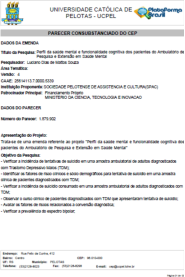
\includegraphics[width=.9\textwidth]{img/cartacep01.pdf}
        \end{center}

        \begin{center}
        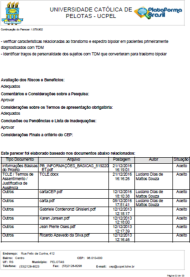
\includegraphics[width=.9\textwidth]{img/cartacep02.pdf}
        \end{center}

        \begin{center}
        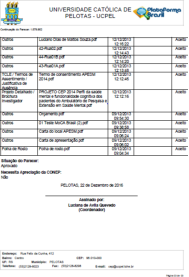
\includegraphics[width=.9\textwidth]{img/cartacep03.pdf}
        \end{center}

\end{anexosenv}


\end{document}
